Neste capitulo será detalhado o framework Searchlight e os recursos que o mesmo oferece para seus usuários.

\section{Website do projeto}
Pensando em ilustrar os recursos do framework Searchlight, para os usuários do framework, foi criado um website com informações do projeto.

O endereço dele é \url{http://wancharle.github.io/Searchlight/}. Através dele podemos ter acesso ao endereço do código fonte do projeto, que se encontra no GitHub, permitindo assim que outros programadores contribuam para o mesmo.

\begin{figure}[htb]
	\caption{\label{fig-website}Website com documentação e exemplos do Framework Searchlight.}
	\begin{center}
	    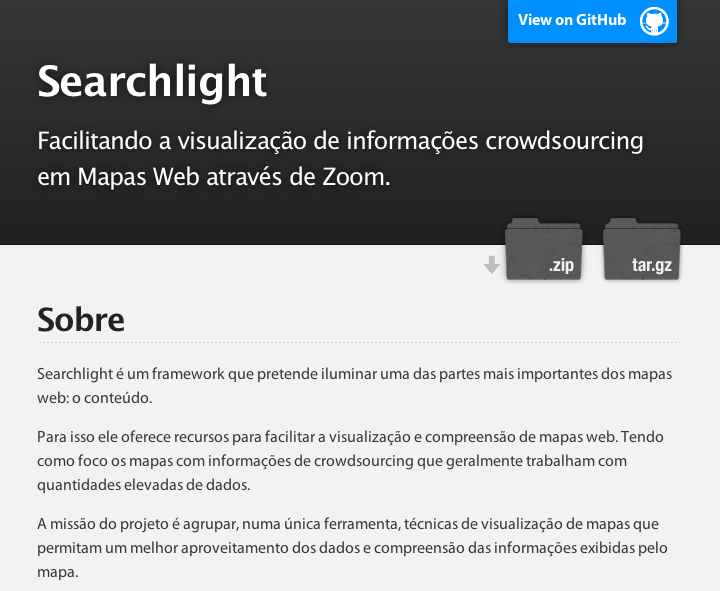
\includegraphics[scale=0.6]{website}
	\end{center}
\end{figure}


Este website contém o link da API Searchlight.js para os programadores que querem utilizar o framework de forma customizada. Nele é possível visualizar exemplos de filtros de categorias, agrupamento de marcadores, foco em grupo, geração automática de mapas e compartilhamento de mapas, que são os principais recursos e meios de utilização do framework. Dentre eles, destacam-se a geração e compartilhamento automático de mapas que possuem paginas específicas para sua utilização. 


Em suma, o website documenta o projeto como um todo. Fala sobre os objetivos e metas do projeto. É possivel conferir uma parte do dele na \autoref{fig-website}: 

\section{Recursos desenvolvidos}
A \autoref{sec-estrategias} descreveu duas estratégias que podem ser utilizadas para se lidar com o problema de muitos marcadores num mapa. O framework fornece recursos que se baseiam nessas duas estratégias. 

\subsection{Filtro por categorias}
O filtro por categoria é um dos recursos do framework Searchlight que se baseia na estratégia de redução de marcadores. Através dele é possível selecionar quais categorias de informações devem ser exibidas pelo mapa. 

Para utilizar o filtro por categorias basta que o usuário acesse o menu Searchlight, localizado no campo superior direito do mapa, faça a escolha de quais categorias devem ser exibidas e clique no botão atualizar mapa. 

\begin{figure}[htb]
	\caption{\label{fig-categorias}Filtro por categoria fornecido pelo framework Searchlight}
	\begin{center}
	    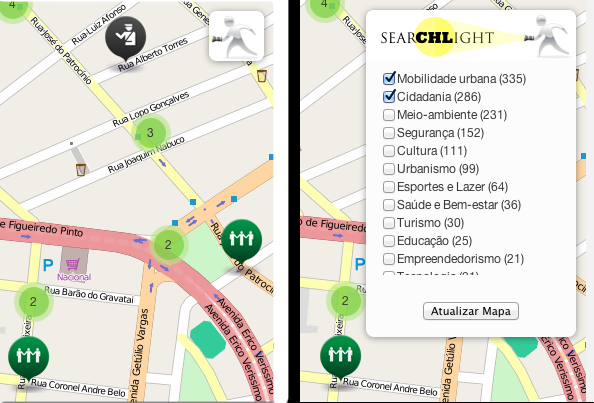
\includegraphics[scale=0.6]{categorias}
	\end{center}
\end{figure}

A \autoref{fig-categorias} exibe o processo de visualização do filtro por categorias.
Como pode ser observado, o filtro  exibe um número ao lado de cada categoria. Este número representa o quantidade de marcadores que pertencem a categoria.

É importante ressaltar, que o filtro de categorias é gerado dinamicamente através da leitura dos dados do mapa. Se os dados utilizados pelo mapa não forem classificados por categoria o filtro não é exibido.

\subsection{Agrupamento de marcadores}	
Outra recurso interessante fornecido pelo framework Searchligth é o agrupamento de marcadores. Por meio, da biblioteca Leaflet.MarkerCluster o framework agrupa os marcadores de acordo com o nível de zoom. Isto, somente, já resolve o problema de sobreposição de informações que é um dos problemas que motivaram a criação deste projeto. 

Outro problema que também é resolvido pelo agrupamento de marcadores é o problema de zoom arbitrário. Pois, quando o usuário clica em um agrupamento de marcadores o mapa calcula um nível de zoom em que é possível ver todos os subelementos do agrupamento que foi clicado. A \autoref{fig-agrupamentos} exemplifica isso. Com apenas um clique no marcador central o mapa pula do zoom A para o zoom B sem precisar de zoons intermediários como no caso analisado na \autoref{fig-zoomab}.


\begin{figure}[htb]
	\caption{\label{fig-agrupamentos}No framework Searchlight os agrupamentos de marcadores eliminam o zoom arbitrário}
	\begin{center}
	    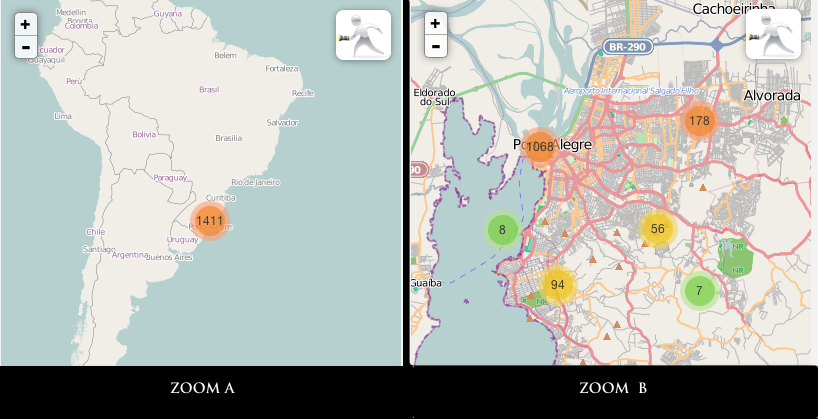
\includegraphics[scale=0.5]{agrupamentos}
	\end{center}
\end{figure}


\subsection{Balões de Resumo e Foco em grupo}
Em mapas com um elevado número de  categorias seria interessante que o framework exibi-se algum recurso visual para resumir a informação de cada agrupamento de marcadores. 
No framework Searchlight isto foi implementado através de balões de resumo.

A \autoref{fig-baloes} exibe um balão de resumo. Como pode se observar, o Balão de resumo exibe um pequeno relatório sobre os elementos pertencentes ao agrupamento. É exibido uma listagem de ícones de categorias, que pertencem ao agrupamento que foi clicado, com o total de elementos da categoria em baixo do ícone. 

\begin{figure}[htb]
	\caption{\label{fig-baloes}Balãoes de Resumo do agrupamento clicado}
	\begin{center}
	    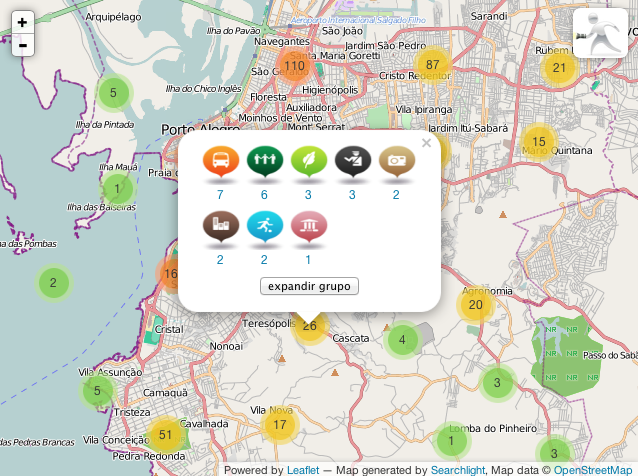
\includegraphics[scale=0.6]{baloes}
	\end{center}
\end{figure}

Balões de Resumo fornecem duas formas de interação. A primeira forma de interação é com o botão "expandir grupo" que basicamente faz um zoom no grupo. A segunda forma de interação é com os icones de categorias. Através dele é possível utilizar o recurso "Foco em Grupo" que basicamente faz um zoom no grupo, mas exibindo apenas os elementos pertencentes ao agrupamento e a categoria que foi clicada.

O recurso de foco em grupo é útil para situações que se deseja visualizar apenas um tipo de categoria de forma rapida sem que seja preciso marcar e desmarcar categorias no filtro de categorias. Para sair do foco em grupo basta clicar no botão DESFOCAR. Veja \autoref{fig-focoemgrupo}.

 \begin{figure}[htb]
	\caption{\label{fig-focoemgrupo}Exemplo de Foco em Grupo por categoria segurança}
	\begin{center}
	    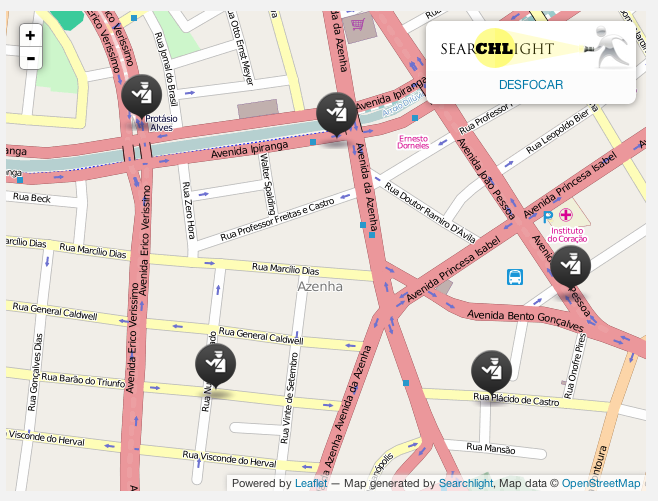
\includegraphics[scale=0.6]{focoemgrupo}
	\end{center}
\end{figure}


\subsection{Geração e Compartilhamento automático de Mapas}

